\section*{Problem 3 (50') (Low Diameter Decomposition)} 
In this problem, you'll learn Low Diameter Decomposition, and use it to give approximate algorithm for some fundamental graph problem like Tree Embedding, All Pair Shortest Path (APSP).

\textcolor{red}{In this problem, the graph can be seen as weighted graph with all the weight being positive integer. }
\begin{definition}[Low Diameter Decomposition (LDD)]
    Given an undirected graph $G = (V, E)$, a \textbf{Low Diameter Decomposition (LDD)} scheme with approximation factor $\beta$ and diameter bound $D$ is a randomized algorithm that partitions $V$ into disjoint clusters $V_1, V_2, \dots, V_k$ satisfying:
    \begin{enumerate}
        \item \textbf{Bounded Diameter}: For each $V_i$, the diameter of $G[V_i]$  $\leq D$.
        \item \textbf{Separation Probability}: For any $x, y \in V$,
        $$
            \Pr\big[\text{$x$ and $y$ lie in different clusters}\big] \leq \beta \cdot \frac{d_G(x, y)}{D},
        $$
        where $d_G(x, y)$ denotes the shortest-path distance between $x$ and $y$ in $G$.
    \end{enumerate}
\end{definition}

\noindent \textbf{Remarks}:
\begin{itemize}
    \item The \textbf{diameter} of $G[V_i]$ is $\max_{u,v \in V_i} d_{G}(u, v)$.
    \item $\beta$ balances cluster tightness ($D$) and separation likelihood. Lower $\beta$ implies better decomposition quality.
\end{itemize}

    \begin{itemize}
        \item [a. (10')] Prove that the following algorithm gives a LDD with approximation factor $\beta = O(\log n)$, with probability $\ge 1 - n ^ {-1}$.
\begin{algorithm}[H]
\caption{Low Diameter Decomposition (LDD)}
\label{alg:ldd}
\begin{algorithmic}[1]
\Require Undirected graph $G=(V,E)$, target diameter $D > 0$
\Ensure Vertex partition $\{V_1,\dots,V_k\}$ with $\mathrm{diam}(G[V_i]) \leq D$
\State Initialize $\mathit{marked}[v] \gets \textsc{False}$ for all $v \in V$
\While{$\exists v \in V$ with $\neg\mathit{marked}[v]$}
    \State Select arbitrary unmarked vertex $v_0 \in V$
    \State \textcolor{red}{Sample $R_{v_0} \sim \mathrm{Geometric}(p)$ with $p = \min\big(1, \frac{4\log_e n}{D}\big)$.}
    \State \textcolor{red}{Compute $B \gets \{u \in V \mid \lnot marked[u] \land  d_G(v_0,u) \leq R_{v_0}\}$}
    \State Create cluster $C \gets B$ 
    \State $\mathit{marked}[u] \gets \textsc{True}$ for all $u \in C$
    \State Add $C$ to output partition
\EndWhile
\State \Return the computed clustering
\end{algorithmic}
\end{algorithm}
\noindent \textbf{Remarks}: The naive way to run LDD takes time $O(n ^ 3)$, since one need to run Dijsktra for $n$ times. However, there are ways to do LDD in $\tilde{O}(n ^ 2)$ time. You will get \textcolor{red}{10 Bonus Point} if you can find out. 
    \end{itemize}


We will use this tool to solve approximate APSP problem. First, we will introduce Low Stretch Tree. 


\begin{definition}
    A randomized low-stretch tree of stretch  $\alpha$ for a graph $G=(V,E)$ is a probability distribution $\mathcal{D}$ over spanning trees of $G$ s.t.
    \begin{enumerate}
        \item $d_G(x, y) \le d_T(x, y)$, for all $T$ in the support $\mathcal{D}$.
        \item $\E_{T\sim \mathcal{D}}[d_T(x, y)] \le \alpha \cdot d_G(x,y)$, $\forall x, y \in V$
        
    \end{enumerate}
\end{definition}

\begin{theorem}\label{LST}
    For any metric space $M=(V, d)$, there exists an efficiently sampleable $\alpha_B$-stretch spanning tree distribution $\mathcal{D}_B$, where

$$
\alpha_B=O\left(\log n \log \Delta_M\right)
$$

$\Delta_M$ is defined as $\max_{x, y} d(x, y)$, we assume $\forall x\neq y, d(x, y) \ge 1$. 

\end{theorem}

We will prove theorem \ref{LST} by the following algorithm. 

\begin{algorithm}[H]
\caption{Low Stretch Tree Construction, LST$(M, \delta)$}
\label{alg:lst}
\begin{algorithmic}[1]
\Require Metric space $M=(V,d)$, target diameter $D=2^\delta$
\Ensure Spanning tree $T$ with low stretch.  \textbf{Invariant}: $\mathrm{diameter}(M) \leq 2^\delta$
\If{$|V| = 1$}
    \State \Return trivial tree containing the single point
\EndIf
\State Partition $V$ into clusters $C_1,\dots,C_t \gets \mathrm{LDD}(M, D/2)$ 
\For{$j = 1$ \textbf{to} $t$}
    \State Let $M_j$ be $M$ restricted to $C_j$
    \State Recursively build $T_j \gets \mathrm{LST}(M_j, \delta-1)$
\EndFor
\State Connect roots $r_2,\dots,r_t$ to $r_1$ with edges of length $2^\delta$
\State \Return final tree $T$ rooted at $r_1$
\end{algorithmic}
\end{algorithm}

\begin{lemma}\label{lemLST}
    If the random tree $T$ returned by some call LST($M, \delta$) has root $r$, then 
    \begin{enumerate}
        \item every vertex $x$ in $T$ has distance $d_{\textcolor{red}{T}}(x, r) \le 2 ^ {\delta + 1}$
        \item the expected distance between any $x, y\in T$ has $\E[d_T(x, y)] \le 8 \delta \beta d(x, y)$. (Recall that $\beta$ is the approximate factor in LDD) 
    \end{enumerate}
\end{lemma}

If we can prove Lemma \ref{lemLST}, then one can see from Problem a that if $\beta = O(\log n)$, then with high probability, $d_T(x, y) \ge d(x, y)$ for any $x, y$, thus theorem \ref{LST} can be proved. 


    \begin{itemize}
        \item [b. (20')] Prove the Lemma \ref{lemLST}. 
    \end{itemize}


    
    \begin{itemize}
        \item [c. (10')] Prove the following theorem. 

        \begin{theorem}
            There's an algorithm that output $O(\log n\log \Delta)$ approximation of APSP on an undirected graph in $\tilde{O}(n ^ 2)$ time, and success with probability $\ge 1 - \frac 1{\text{poly}(n)}$.
        \end{theorem}


        (This means, the algorithm output $d'(x, y)$ for any pair $x, y$, and satisfies $d(x, y) \le d'(x, y) \le \log n\log \Delta \cdot d(x, y)$, where $d(x, y)$ is the length of shortest path between $x, y$. )
    \end{itemize}

    % Actually, one can directly use LDD to get an approximate algorithm for ASAP, and achieve $O(\log n)$ approximation. 
    \begin{itemize}
        \item [d. (10')] Prove the following theorem. 

        \begin{theorem}
            There's an algorithm that output $O(\log n)$ approximation of ASAP on an undirected graph in $\tilde{O}(n ^ 2)$ time, and success with probability $\ge 1 - \frac 1{\text{poly}(n)}$.
        \end{theorem}
    \end{itemize}

\newpage
\begin{answer}
    \begin{enumerate}[label=\alph*).]
        \item We first prove the diameter bound by showing that $R_{v_0} \le D/2$ with high probability and then using 
        the triangle inequality to bound the diameter of cluster $V_i$, i.e. for any $u, v \in V_i$, we have
        \begin{align*}
            d_G(u, v) &\le d_G(u, v_0) + d_G(v_0, v) \le \frac{D}{2} + \frac{D}{2} = D.
        \end{align*}
        Now compute the probability that $R_{v_0} > D/2$ for a given cluster $V_i$:
        \begin{align*}
            \Pr[R_{v_0} > D/2] = (1 - p)^{D/2} \le e^{-pD/2} \le e^{-2\log n} = \frac{1}{n^2}.
        \end{align*}
        Here we use $1 - x \le e^x$ for all $x \in \mathbb{R}$. Then by union bound, we have
        \begin{align*}
            \Pr\left[\exists \text{a cluster with diameter} > D\right] &= 1 - \Pr\left[\exists v\in V, R_{v_0} > D/2\right] \\
            &\ge 1 - \frac{n}{n^2} = 1 - \frac{1}{n}.
        \end{align*}
        Then we bound the separation probability using the memoryless property of geometric distribution. For any $x, y \in V$, 
        assume the center vertex picked is $v$. Sampling $R_{v}$ from $\mathrm{Geometric}(p)$ can be seen as flip a coin of bias $p$ until we get a head.
        Without loss of generality, assume $x$ will lie in the current ball first. At this time, we have flipped $d_G(v,x)$ coins without seeing a head. 
        
        Then the case that $x$ and $y$ lie in different clusters will happen if we see a head within the next $d_G(v,y) - d_G(v,x) \le d_G(x,y)$ flips. 
        Therefore, 
        \begin{align*}
            \Pr[x, y \text{ lie in different clusters}] &= \Pr[R_v < d_G(v,y) | R_v \ge d_G(v,x)] \\
            &= 1 - \Pr[R_v \ge d_G(v,y) | R_v \ge d_G(v,x)] \\
            &= 1 - \Pr[R_v \ge d_G(v,y)-d_G(v,x)] \\ 
            &= 1 - (1-p)^{d_G(v,y)-d_G(v,x)}  \\
            (d_G(v,y) - d_G(v,x) \le d_G(x,y))\quad&\le 1 - (1-p)^{d_G(x,y)} \\
            (\forall p \in [0,1],(1-p)^x \ge 1-px) \quad&\le 1 - ( 1 - p\cdot d_G(x,y)) = p\cdot d_G(x,y) \\
            &\le 4\log n \cdot \frac{d_G(x,y)}{D}  = O(\log n) \cdot \frac{d_G(x,y)}{D}.
        \end{align*}
        Notice that if $(x,y) \notin E$, we can repeat the above argument along the shortest path from $x$ to $y$ in $G$, and the results still hold.

        \textcolor{blue}{\textbf{Bonus. It seems that the there are problems in following algorithm but I didn't find better way :(.}}
        The basic idea is reducing redundant queries to the same vertex.
        \begin{algo}
            \caption{Improved Low Diameter Decomposition (LDD) with $\tilde{O}(n^2)$ time complexity}
            \label{alg:improved-ldd}
            \begin{algorithmic}[1]
            \Require Undirected graph $G=(V,E)$, target diameter $D > 0$
            \Ensure Vertex partition $\{V_1, \dots, V_k\}$ with $\mathrm{diam}(G[V_i]) \leq D$
            \State Initialize $\mathit{marked}[v] \gets \textsc{False}$ for all $v \in V$
            \While{$\exists v \in V$ with $\neg\mathit{marked}[v]$}
                \State Select arbitrary unmarked vertex $v_0 \in V$
                \State Sample $R_{v_0} \sim \mathrm{Geometric}(p)$ with $p = \min\big(1, \frac{4\log_e n}{D}\big)$
                \State $\mathit{marked}[v_0] \gets \textsc{True}$
                \State \textcolor{red}{\textbf{Initialize an empty priority queue $Q$ and add $v_0$ with distance $0$.}} \Comment{Use BFS}
                \While {$Q$ is not empty}
                    \State \textcolor{red}{\textbf{Pop the vertex $u$ with the smallest distance $d_u$ from $Q$}}
                    \If{$\neg\mathit{marked}[u]$}
                        \State $\mathit{marked}[u] \gets \textsc{True}$
                        \State Add $u$ to cluster $C$
                    \EndIf
                    \For{each neighbor $w$ of $u$}
                        \If{$\neg\mathit{marked}[w]$ and $d_G(v_0, w) + d_u \le R_{v_0}$}
                            \State \textcolor{red}{\textbf{Add $w$ to $Q$ with distance $d_G(v_0, w)+ d_u$}}
                        \EndIf
                    \EndFor
                \EndWhile
            \EndWhile
            \State \Return the computed clustering
            \end{algorithmic}
        \end{algo}
        \textbf{Time complexity}: notice that each vertex will be added and poped from the priority queue only once.
        And in line 12, each vertex will be queried by its neighbors at most $\text{deg}(u)$ times and $\sum_{v \in V} \text{deg}(v) = O(m) = O(n^2)$. 
        We use heap-based priority queue whose time complexity of poping and adding is $O(\log n)$. 
        
        Therefore, the total time complexity of the algorithm is $O(m + n\log n) = O(n^2 + n\log n) = \tilde{O}(n^2)$.

        \textbf{\textcolor{red}{Note:} We can use algorithm (CKR Decomposition) in Figure \ref{fig:ckr} with better bound and $\tilde{O}(n^2)$ time complexity instead of the above algorithm.}
        \item We will prove the lemma by induction on $\delta$. 
        
        \textbf{Base case}: when $\delta = 0$, we have $|V| = 1$ and the tree is a single vertex. There is nothing to prove.
        Assume the lemma holds for $\delta - 1$ and consider the case $\delta$ as follows:
        
        \textbf{Induction step}: We prove the fisrt part of the lemma first.
            Consider $x$ lies in cluster $C_i$ (denote the corresponding tree as $T_i$) and by the induction hypothesis, $d_{T_i}(x, r_i) \le 2^{\delta}$. 
            And the distance to the new root $r$ is at most $2^{\delta}$ more. $d_{T}(x, r) \le d_{T_i}(x, r_i) + 2^{\delta} \le 2^{\delta + 1}$.
            So the first part of the lemma holds.

            Now we prove the second part of the lemma. According to the part(a), we know that for any $x, y$, 
            \begin{align*}
                \Pr[x, y \text{ is separated }] \le \beta\cdot \frac{d_{G}(x,y)}{2^{\delta-1}}
            \end{align*}
            And if $x$ and $y$ are in the same cluster(denote as $T_i$), by the induction hypothesis, we have
            \begin{align*}
                \E[d_{T_i}(x,y)] \le 8\beta(\delta - 1) d_{G}(x,y).
            \end{align*}
            Therefore, the expected distance between $x$ and $y$ is
            \begin{align*}
                \E[d_T(x,y)] &\le \Pr[x, y \text{ is separated }] \cdot (d_T(x, r) + d_T(y, r)) \\
                & \quad \quad \quad \quad + \Pr[x, y \text{ is not separated }] \cdot d_{T_i}(x,y) \\
                &\le \beta\cdot \frac{d_{G}(x,y)}{2^{\delta-1}} \cdot \left(2^{\delta + 1} + 2^{\delta + 1}\right) + 8\beta(\delta - 1) d_G(x,y) \\
                &= 8\delta\beta\cdot d_G(x,y).
            \end{align*}
            Therefore, the lemma holds for all $\delta$. Then we use the lemma to prove the theorem \ref{LST}. 
            
            \textcolor{blue}{When $\beta = O(\log n)$, we first prove that for $\mathcal{D}_B$ over spanning trees, $d_G(x,y) \le d_T(x,y)$ for any $T$ in  $\text{supp}(\mathcal{D}_B)$.}
            Notice that $d_G(x, y) \le \Delta_M = 2^\delta$ here. Fix $x$ and $y$, and let $i$ such that $d_G(x, y) \in (2^{i-1}, 2^i]$. 
            Then consider the invocation of $\mathrm{LST}(U, i)$ such that $x\in U$.
            \begin{itemize}
                \item If $y \in U$, then by the definition of LDD, $x,y$ will fall into separate clusters with high probability. Therefore, by the procedure of LST, $d_T(x,y) \ge 2^i$, which is the length of the edge connecting different subtrees.
                \item If $y \notin U$, then $x$ and $y$ must be separated at a higher level $i' > i$ during the recursion of LST, hence $d_T(x,y) \ge 2^{i'} > 2^i$.
            \end{itemize}
            In sum, $d_G(x,y) \le d_T(x,y)$ for any $T$ in  $\text{supp}(\mathcal{D}_B)$. 

            And due to $\delta = \log(\Delta_M)$, then by the lemma \ref{lemLST}, we have
            \begin{align*}
                \E_{T\sim \mathcal{D}_B}[d_T(x,y)] &\le 8\delta\beta d_G(x,y) = O(\log n \log \Delta_M) d_G(x,y). \forall x,y \in V.
            \end{align*}
            which concludes the proof of theorem \ref{LST}.
        \item We have proven that theorem \ref{LST} holds for any metric space $M$. Then the \textbf{Algorithm \ref{alg:ldd}} is an approximate algorithm for APSP with factor $O(\log n \log \Delta)$ where $\Delta := \max_{x,y} d(x,y)$.
        The correctness is guaranteed by theorem \ref{LST}. 

        \textbf{Time complexity}: We use the improved LDD algorithm whose time complexity is $\tilde{O}(n^2)$.
        Denote the total time complexity of the algorithm as $T(n)$, then 
        \begin{align*}
            T(n) = \tilde{O}(n^2) + \sum_{i=1}^t T(n_i) \text{ where } \sum_{i=1}^{t} n_i = n 
        \end{align*} 
        which implies that each level of recursion takes at most $\sum_{i=1}^{t} \tilde{O}(n_i^2) = \tilde{O}(n^2)$ time.

        Notice that the depth of recursion is at most $\lceil \log \Delta_M \rceil + 1$. Therefore, the total time complexity is $\tilde{O}(n^2\log \Delta_M) = \tilde{O}(n^2)$.
        \item We try to improve the Algorithm \ref{alg:lst} from $\alpha_B = O(\log n \log \Delta_M)$ to $\alpha_B = O(\log n)$ by introducing a better graph decomposition method called 
        \textbf{CKR Decomposition}~\cite{CKR_Decomposition}.
        \begin{algo}
            \caption{CKR Decomposition}
            \label{alg:ckr}
            \begin{algorithmic}[1]
                \Require{Undirected graph $G=(V,E)$, distance metric $d$ and $D$}
                \Ensure{Vertex partition $\{V_1, \dots, V_k\}$.}
                \State Randomly sample $R \sim \text{Uniform}[D/4, D/2]$.
                \State Choose a random permutation $\pi: V \to V$ uniformly at random.
                \State Initialize $\mathit{marked}[v] \gets \textsc{False}$ for all $v \in V$
                \For{$v_0$ in the order given by $\pi$}
                    \If{$\mathit{marked}[v_0]$}
                        \State continue     \Comment{Skip if already covered by previous clusters}
                    \EndIf
                    \State Compute $C \gets \{u \in V \mid \lnot marked[u] \land  d_G(v_0,u) \leq R_{v_0}\}$
                    \State $\mathit{marked}[u] \gets \textsc{True}$ for all $u \in C$
                    \State Add $C$ to output partition
                \EndFor
                \State \Return the computed clustering
            \end{algorithmic}
        \end{algo}
        we can implement CKR Decomposition in $\tilde{O}(n^2)$ time with priority queue instead of the naive Dijkstra algorithm \cite{mendel2009fastckrpartitionssparse}. 
        The detailed algorithm shows in \textbf{Figure \ref{fig:ckr}} and the time complexity is $O(m\log n  + n\log^2 n) = \tilde{O}(n^2)$.
        \begin{figure}[htbp]
            \centering
            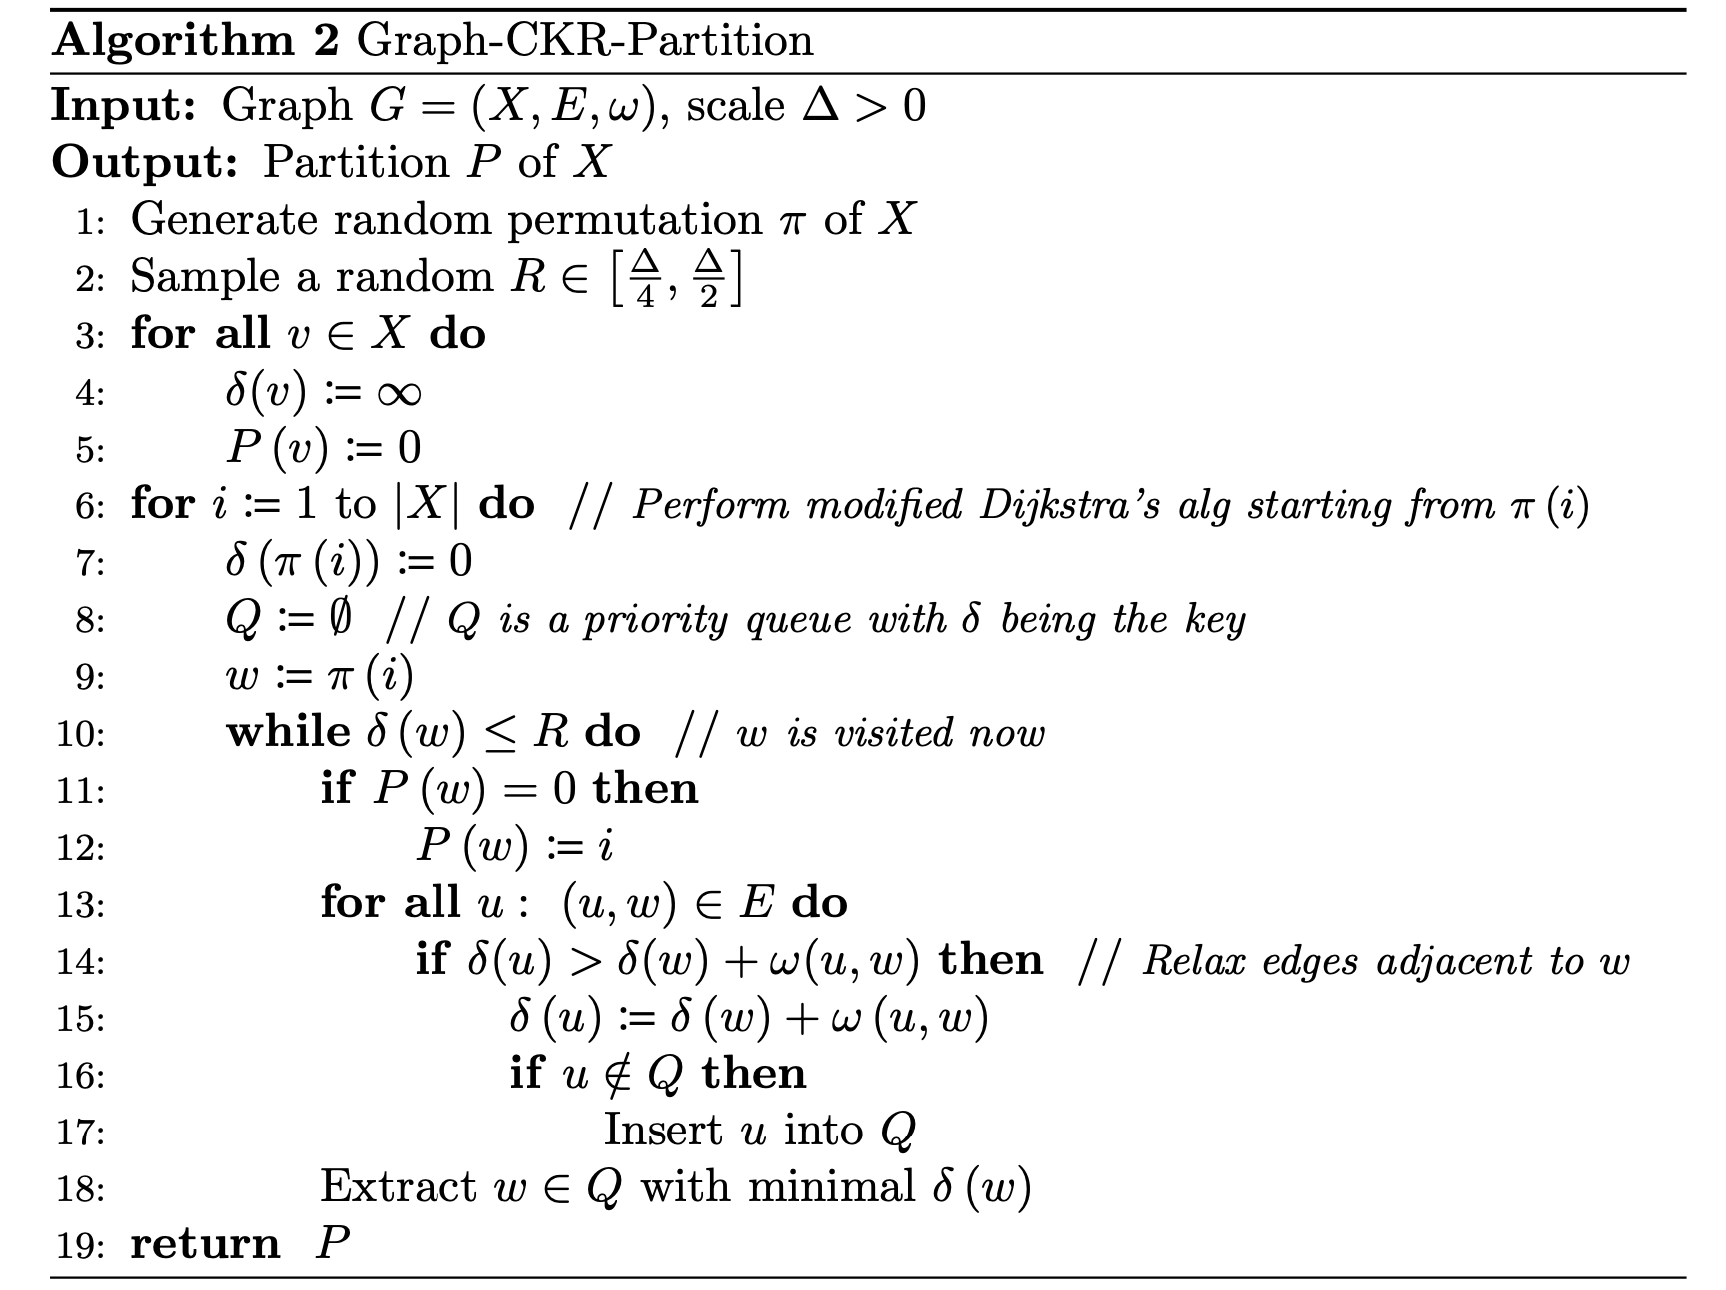
\includegraphics[width=0.9\textwidth]{./images/Graph-CKR.png}
            \caption{Fast CKR Decomposition Algorithm proposed in \cite{mendel2009fastckrpartitionssparse}.}
            \label{fig:ckr}
        \end{figure}

        Then we  prove CKR Decomposition has \textbf{Bounded Diameter} and \textbf{Separation Probability}:
        
        Bounded diameter is satisfies by the definition of CKR Decomposition directly(see line 1), i.e. we have 
            $\forall C_i$, there exists $c_i \in C_i$ such that $d_G(c_i, u) \leq D/2$ for all $u \in C_i$ which implies that $d_G(u, v) \leq D$ for all $u, v \in C_i$.
        
        Then for any $u, v \in V$, reorder the vertexs as $w_1, w_2, \cdots, w_n$ according to $\min\{d(w_i, u), d(w_i, v)\}$.
        Without loss of generality, denote $d(w_j, u) := a_j$, $d(w_j, v) := b_j$ and assume $a_j < b_j$.
        Then the case that $u$ is in $w_j$'s cluster and $v$ is not need to satisfy (1) $R \in [a_j, b_j]$, (2) $w_j$ appears before $w_{1}, \cdots, w_{j-1}$ in the order given by $\pi$ (Otherwise, $u$ will be assigned cluster before $w_j$'s). Thus, 
        \begin{align*}
            \Pr\left[u,v \text{ is separated}\right] &\le \sum_{i=1}^{n} \Pr\left[ \text{$u$ is in $w_i$'s cluster and $v$ is not}\right] \\
            &\le \sum_{i=1}^{n} \Pr\left[R \in [a_i, b_i]\right] \cdot \Pr\left[\text{$w_i$ appears before $w_{1}, \cdots, w_{i-1}$}\right] \\
            \text{(triangle inequality.)} &\le \sum_{i=1}^{n} \frac{d_G(u, v)}{D/2 - D/4} \cdot \frac{1}{i} = \frac{d_G(u, v)}{D/4} \cdot \sum_{i=1}^{n} \frac{1}{i} \\
            &= O(\log n)\frac{d_G(u, v)}{D}.
        \end{align*}
        In order to achieve $O(\log n)$ approximation in LST, we can analyze the probability more carefully to get a better bound\footnote{The detailed analysis is interesting but hard. Here I refer many materials like \cite{CKR_Decomposition}, \cite{mendel2009fastckrpartitionssparse} and \href{https://www.cs.cmu.edu/~15850/}{notes of CMU course}.}. 
        \begin{align}
            \label{eq:ckr-separation}
            \Pr[u, v \text{ is separated}] \le \frac{d_G(u,v)}{D/4} \cdot \log\left(\frac{\# B(u, D)}{\# B(u, D/8)}\right)
        \end{align}
        where $B(x, r):= \{y: d_G(x,y) \le r\}$. The proof idea is that suppose $d_G(u,v) < D/8$ (Otherwise, the probability of separability is at most $8d_G(u,v)/D$ which is greater than 1 already.)
        Assume $u$ is closer to $w_j$ than $v$, then $d_G(u, w_i) \le D$ and $d_G(u, w_i) \ge D/4 - d_G(u, v) \ge D/8$. Combine the new restriction and two requirements above, we can get the better bound.

        Then we replace the LDD in Algorithm \ref{alg:lst} with CKR Decomposition and get a new algorithm for APSP, and we can prove $\alpha_B = O(\log n)$ here.

        The first part, i.e. $d_G(x, y) \le d_T(x, y)$, for all $T$ in the support $\mathcal{D}$. The proof is almost the same as the one in part (b) of this problem \textcolor{blue}{(see the last few lines in page 9, marked in blue)}.

        Then we prove the following theorem: 
        \begin{theorem}[\cite{FRT_Approximation}]
            \label{thm:ckr}
            Replace the LDD in Algorithm \ref{alg:lst} with CKR Decomposition, then for all $x, y \in V$, we have
            \begin{align*}
                \E_{T\sim \mathcal{D}}[d_T(x, y)] \le O(\log n) \cdot d_G(x,y)
            \end{align*}
        \end{theorem}       
        The proof is similar to the one in part (b) of this problem, here we only show the most important part. 
        Using induction we have: (level $i$ means LST$(M, i)$)
        \begin{align*}
            \E_{T\sim \mathcal{D}}[d_T(x, y)] &= \sum_{i=\delta}^{0} \Pr[x, y\text{ are separated at level } i] \cdot \left(2^{i+1} + 2^{i+1}\right) \\
            (\text{Apply \eqref{eq:ckr-separation}}) &\le  \sum_{i=\delta}^{0} \frac{d_G(u,v)}{2^{i-1}/4} \cdot 4\cdot 2^i \cdot \log\left(\frac{\# B(u, 2^{i-1})}{\# B(u, 2^{i-4})}\right) \\
            &= 32 \cdot d_G(x,y) \sum_{i=\delta}^{0} \log (\# B(u, 2^{i-1})) - \log (\# B(u, 2^{i-4})) \\
            &= 32 \cdot d_G(x,y) \sum_{i=\delta}^{\delta-2} \log (\# B(u, 2^{i-1})) \\
            &\le 96 \cdot d_G(x,y) \log n
        \end{align*}    
        where the last inequality is due to the fact that $\# B(u, 2^{i-1}) \le n$ for all $i$.

        In sum, theorem \ref{thm:ckr} holds. Therefore, the LST algorithm with CKR Decomposition can achieve $O(\log n)$ approximation for APSP. 
        And due to the \textbf{Algorithm \ref{alg:ckr} (CKR Decomposition)} can be implemented in $\tilde{O}(n^2)$ time just like LDD, the total time complexity of the algorithm is $\tilde{O}(n^2)$ as well.
    \end{enumerate}
    \ed
\end{answer}